\section{ Data Warehouse}
\subsection{O que é um Data Warehouse}
Para \citeauthor{jmj} (\citeyear{jmj}), um \textit{Data Warehouse} é um repositório de informação coletada de múltiplas fontes, armazenados sobre um esquema definido e, geralmente, situado em um único local, no intuito de garantir a consistência dos dados caso eles sejam acessados de locais diferentes. Eles suportam o processamento de informações ao prover uma plataforma sólida de dados históricos para análise \citep{jmj}.

\subsection{Características de um Data Warehouse}
Segundo Inmon(1996), um DW é um conjunto de dados orientado por assuntos, integrado, variável com o tempo e não volátil, criados para dar suporte à decisão.

Orientado por assunto, ou seja, organizado em torno de um assunto principal. Ao invés de se concentrar nas operações diárias e no processamento de transações de uma empresa, um DW foca na modelagem e análise de dados para tomadores de decisões \citep{jmj}.
Integrado, um DW contém informações de fontes heterogêneas, como base de dados relacionais e \textit{flat files}. Processos de \textit{data integration} e \textit{data cleaning} são aplicados para garantir consistência dos dados \citep{jmj}.

Variável com o tempo, armazena informações históricas dos últimos 5-10 anos, por exemplo. Toda estrutura chave em um DW contém um elemento de tempo \citep{jmj}.
E por último, não volátil, os dados não precisam ser alterados, já que um DW é fisicamente separado do ambiente operacional. As únicas operações realizadas em um DW são: carga inicial e acesso aos dados \citep{jmj}.

\subsection{Modelos de Data Warehouse}
Segundo \citeauthor{jmj} (\citeyear{jmj}) um DW pode ser dividido em três modelos: \textit{enterprise warehouse}, \textit{data mart} e \textit{virtual warehouse}.

\subsubsection{Enterprise Warehouse}
Para \citeauthor{jmj} (\citeyear{jmj}), um \textit{enterprise warehouse} coleta informações sobre um assunto que abrange toda uma organização. Ele fornece integração de dados em escala corporativa, geralmente de um ou mais sistemas operacionais ou de provedores de informação externos. Ele contém dados detalhados e sumarizados e podem variar de alguns poucos gigabytes para centenas de gigabytes.

Um \textit{enterprise warehouse} é um conglomerado das \textit{data warehouse staging} e \textit{presentation areas} de uma organização \citep{kimball2002}


\subsubsection{Data Mart}
Segundo \citeauthor{jmj} (\citeyear{jmj}) um \textit{data mart} contém um subconjunto de dados de uma escala corporativa e tem o escopo limitado a assuntos específicos.

Os \textit{data marts} são geralmente implementados em servidores de baixo custo e tem o seu ciclo de implementação medido em semanas, ao invés de meses ou anos. Os dados podem ser independentes ou dependentes. Caso sejam independentes, os dados tem como fonte um ou mais sistemas operacionais ou provedores de informação externos. No caso de serem dependentes, os dados contidos no \textit{data mart} são fornecidos diretamente de um \textit{enterprise warehouse}.

\subsubsection{Virtual Warehouse}
\citeAuthorPageYear{jmj} dizem que as \textit{virtual warehouses} são um conjunto de \textit{views} em cima dos banco de dados operacionais. Eles podem manter um processamento eficiente de queries exibindo apenas alguns dos possíveis sumários. Ele também é de fácil construção.

\subsection{Componentes}

A figura \ref{fig:dwComponents} mostra quais os componentes de um DW e serão explicados com mais detalhes mais abaixo.
\begin{figure}[H]
\centering
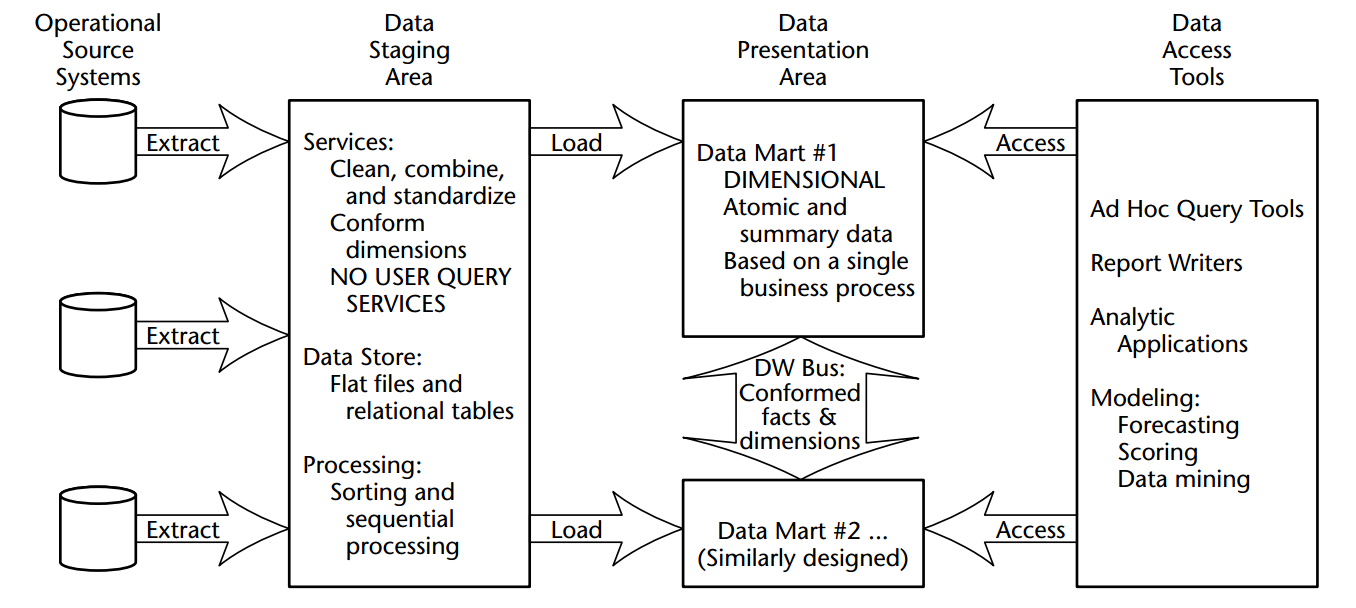
\includegraphics[height=5cm]{imagens/componentes_DW.png}
\caption{Componentes de um Data Warehouse (\citeauthor{kimball2002} \citeyear{kimball2002})}
\label{fig:dwComponents}
\end{figure}

\subsubsection{Operational Source Systems}
Fonte de Dados Operacionais, segundo \citeAuthorPageYear{kimball2013}, são responsáveis pela captura de transações de negócio. Esses sistemas são mantidos fora do \textit{Data Warehouse} por que se tem pouco ou nenhum controle sobre o conteúdo ou formato dos dados. Eles processam performance e disponibilidade. \citeAuthorPageYear{kimball2013} também dizem que esses sistemas mantém poucos dados históricos, um bom \textit{Data Warehouse} pode reduzir a necessidade dos sistemas de dados operacionais de representar o passado. Em muitos casos, eles são de algum propósito especial, sem responsabilidade de compartilhar dados comuns, como dados de produtos, clientes e etc \citeAuthorPageYear{kimball2013}

\subsubsection{Data Staging Area}
\citeauthor{kimball2002} (\citeyear{kimball2002}) dizem que é tanto uma área de armazenamento como um conjunto de processos conhecidos como \textit{extract-transformation-loading} (ETL). Esse processo será melhor explicado mais pra frente. Eles também dizem que a \textit{staging area} é tudo entre os \textit{operational source systems} e a \textit{presentation area}. 

Existem diversas formas de carregar dados na \textit{staging area}, como flat files, xml, modelos relacionais. Ela geralmente é composta de um \textit{database management system} (DBMS) e arquivos de texto (flat files) \citep{kimball2004}. Em muitos casos, os dados precisam ser armazenados fora de um DBMS, em flat files, para um rápido processamento sequencial \citep{kimball2004}.
\citeauthor{kimball2002} (\citeyear{kimball2002}) descrevem o primeiro passo na criação (extração) de um \textit{data staging area} como a leitura e entendimento da fonte de dados e copiar o que for necessário para manipulação futura. Segundo \citeauthor{kimball2002} (\citeyear{kimball2002}), quando os dados são extraídos, existem diversas transformações que podem ser realizadas, como limpeza, combinar dados de diferentes fontes, removendo dados duplicados e etc. Essas transformações acontecem antes de carregar os dados na \textit{presentation area}.

\subsubsection{Data Presentation Area}
A \textit{presentation area}, ou área de apresentação é onde os dados estão organizados, armazenados e disponíveis para consulta por usuários ou alguma aplicação analítica de \textit{Business Intelligence} (BI) \citep{kimball2013}. Tudo que o negócio vê e toca é através dos das ferramentas de acesso ou aplicações de BI.

Os dados devem ser, segundo \citep{kimball2013}, apresentados, armazenados e acessados através de esquemas dimensionais, sejam eles esquemas estrela ou cubos OLAP. Eles também deve conter dados atômicos detalhados \citep{kimball2013}.  Embora a \textit{presentation area} contenha dados agregados, é completamente inaceitável que somente dados sumarizados sejam armazenados enquanto os dados atômicos estão trancados em modelos normalizados. \citep{kimball2013}. Os dados mais finamente granulados devem ser apresentados na \textit{presentation area} para que usuários possam fazer as perguntas mais precisas.

A área de apresentação deve ser estruturada ao redor dos processos de medição de eventos, isso se alinha naturalmente com os \textit{operational source data capture systems}. Os modelos dimensionais devem corresponder aos eventos de captura de dados, não devem entregar um "relatório do dia" (\citeauthor{jmj}, \citeyear{jmj}). 

\subsubsection{Data Access Tools} Ferramentas de Acesso de Dados, ou \textit{Data Access Tools}, são ferramentas usadas para realizar consultas na área de apresentação. Uma ferramenta dessas pode ser tão simples quanto Queries Ad Hoc ou tão complexa quanto uma ferramenta de mineração de dados ou modelagem \citeAuthorPageYear{kimball2013}. 

\subsection{Extract, Transform, Load (ETL)}
O processo de \textit{extract, transform, load} (extrair, transformar, carregar) também conhecido como ETL é um processo utilizado para a construção de um DW, ele contém os passos que são mostrados na figura \ref{etl}. 
\begin{figure}[H]
\centering
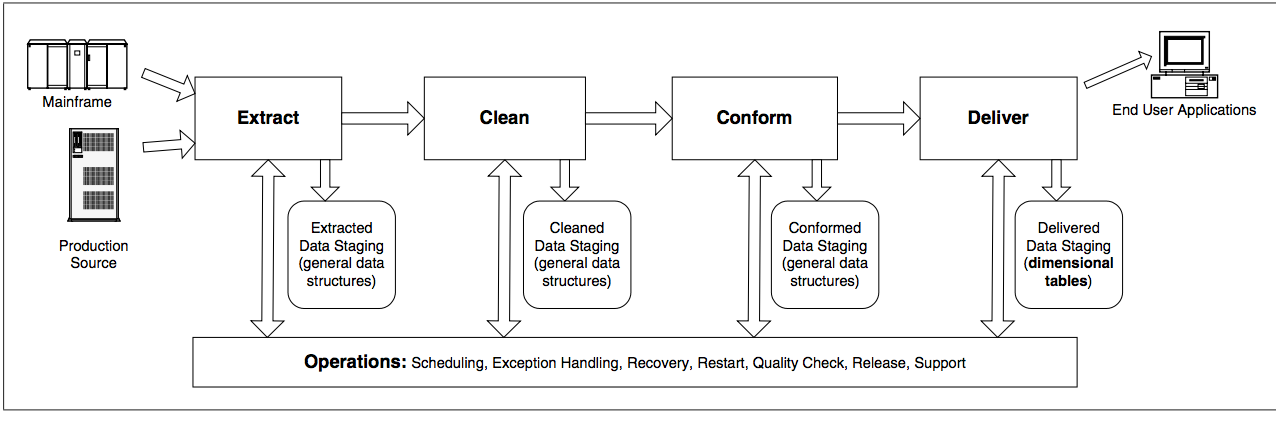
\includegraphics[height=5cm]{imagens/dw_process.png}
\caption{Processo de ETL (\citeauthor{kimball2004} \citeyear{kimball2004})}
\label{etl}
\end{figure}
O primeiro passo é a extração dos dados, é esperado que o sistema tenha que extrair dados de uma grande variedade de fontes \citep{kimball2013}. As organizações podem extrair dados de fontes como arquivos xml, banco de dados, planilhas e etc.

O segundo passo é a transformação, após os dados serem extraídos, diversas transformações podem ser realizadas, como limpeza, combinar dados de fontes diversas e duplicação dos dados \citep{kimball2013}. Essa limpeza pode, segundo \citeauthor{kimball2013} (\citeyear{kimball2013}), mudar os dados e aperfeiçoar o seu valor para uma organização.

O terceiro, e último, passo é o carregamento, que é o processo de estruturar fisicamente e carregar os dados dentro dos modelos dimensionais da \textit{presentation area} \citep{kimball2013}.

\subsection{Modelagem Dimensional}
A modelagem dimensional permite que os usuários do negócio enxerguem os dados com facilidade, ao entregar dados entendíveis e uma performance rápida, com dados visualizados em dimensões.

Existem quatro etapas para a construção de um modelo dimensional, essas são: \textbf{selecionar o processo de negócio}, \textbf{declarar o grão}, \textbf{identificar as dimensões} e \textbf{identificar os fatos}. 

Segundo \citeauthor{kimball2013} (\citeyear{kimball2013}), os processos de negócio são as atividades operacionais realizadas por uma organização. É um processo importante pois define como o grão, dimensões e fatos serão declarados. O grão estabelece o que uma única linha na tabela de fatos representa \citep{kimball2013}.

\subsubsection{Tabela de Dimensões}
De acordo com \citeauthor{kimball2013} (\citeyear{kimball2013}), as dimensões fornecem o contexto de "quem, o que, onde, quando e como" de cada processo do negócio. As tabelas de dimensões podem conter diversas colunas mas geralmente tem menos dados que a tabela de fatos. Elas também tem chave primária, que vai permitir o relacionamento com a tabela de fatos.
\citeauthor{kimball2013} \citeyear{kimball2013} afirmam que a tabela de dimensões pode ser conhecida como a "alma" de um sistema de DW, pois contém dados que permitem que o sistema de DW seja alavancado.

\subsubsection{Tabela de Fatos}
A tabela de fatos armazena as métricas resultantes de um processo de negócio de uma organização (\citeauthor{kimball2013}  \citeyear{kimball2013}). Cada linha em uma tabela de fatos representa um evento de medição. Os dados, em um nível especifico de detalhe, pode ser chamado de grão, como apenas uma linha por produto vendido \citep{kimball2013}.

Os dados que mais úteis são os numéricos e aditivos. Aditividade é importante, pois dificilmente irá se fazer uma consulta que traga apenas uma linha, mas sim irá trazer centenas, milhares ou milhões de dados e a coisa mais útil para se fazer com eles é somar \citep{kimball2013}.

\citeAuthorPageYear{kimball2013} dizem que também é possível manter dados textuais em uma tabela de fatos, eles são comumente usados para descrever algo e estão em uma lista discreta de valores. 

As tabelas de dimensões, segundo \citeAuthorPageYear{kimball2013} tem uma ou mais chaves estrangeiras, que irá ligar as chaves primarias das tabelas de dimensões. Eles também afirmam que a tabela de fatos também tem sua própria chave estrangeira, que é um subconjunto das chaves estrangeiras, chamado de chave composta. 

\subsubsection{Esquema Estrela}
Esse esquema, mostrado como exemplo na figura \ref{star}, armazena os dados em uma arquitetura semelhante a uma estrela, onde cada ponta é uma uma dimensão e todas se relacionam com a tabela de fatos, como mostra a figura. \citeAuthorPageYear{jmj} dizem que a tabela de fatos contém chaves para todas as outras tabelas assim como dados de medidas.
\begin{figure}[ht]
\centering
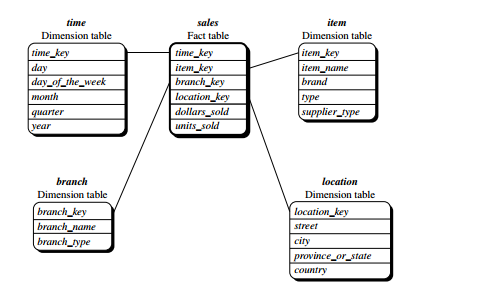
\includegraphics[height=6.2cm]{imagens/starscheme.png}
\caption{Esquema Estrela (\citeauthor{jmj} \citeyear{jmj})}
\label{star}
\end{figure}
\\
\subsubsection{Esquema Snowflake}
Segundo \citeauthor{jmj} \citeyear{jmj}, o esquema \textit{snowflake} é uma variante do esquema estrela onde algumas tabelas de dimensões estão normalizadas, dividindo os dados em tabelas adicionais, como mostra na figura \ref{snowflake}. Eles também dizem que a maior diferença entre o esquema \textit{snowflake} e \textit{star}, é que no snowflake são mantidas normalizadas para evitar redundâncias. Dessa forma fica fácil de armazenar e salva espaço de armazenamento, porém isso pode reduzir a eficacia da exploração, já que mais \textit{joins} precisarão ser feitos para executar a querie \citep{jmj}.
\begin{figure}[ht]
\centering
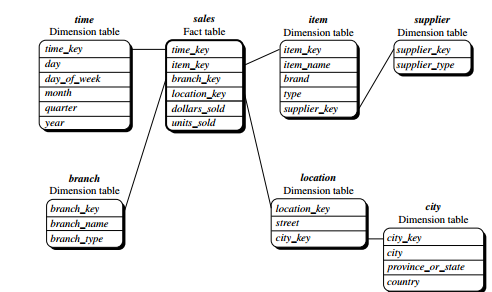
\includegraphics[height=6.2cm]{imagens/snowflakescheme.png}
\caption{Esquema Snowflake (\citeauthor{jmj} \citeyear{jmj})}
\label{snowflake}
\end{figure}
\subsubsection{Cubo e OLAP}
Segundo \citeauthor{jmj} (\citeyear{jmj}), DW e ferramentas OLAP são baseados no modelo multidimensional e esse modelo visualiza os dados no formato de cubos de dados, como mostra a figura \ref{cube}. Um cubo de dados permite visualizar os dados em diversas dimensões simultaneamente.
\begin{figure}[ht]
\centering
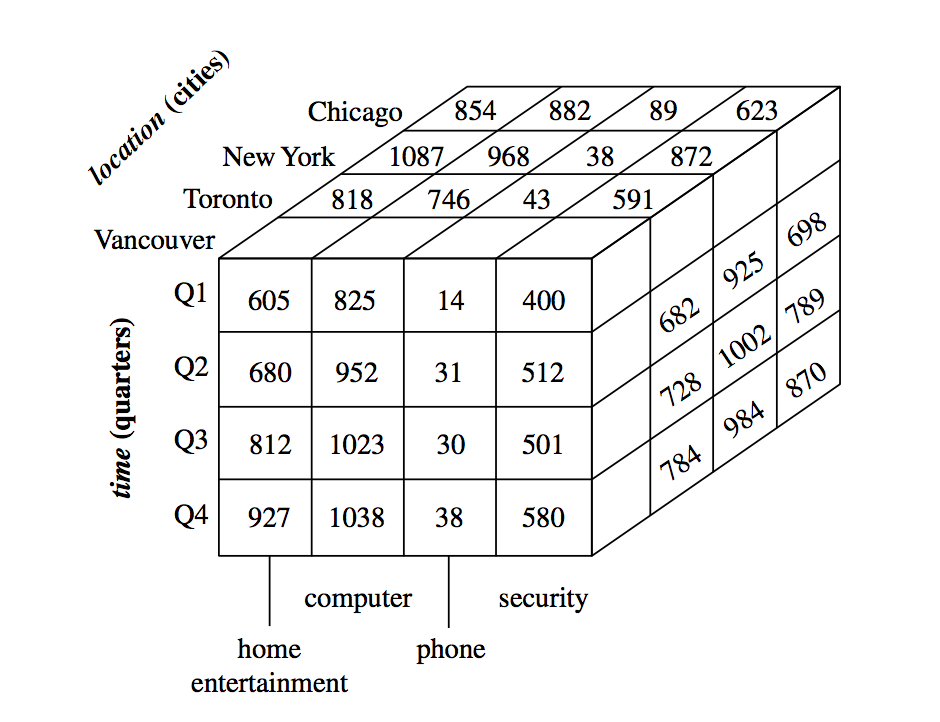
\includegraphics[height=6.2cm]{imagens/datacube.png}
\caption{Exemplo de um cubo de dados (\citeauthor{jmj} \citeyear{jmj})}
\label{cube}
\end{figure}
Dimensões são perspectivas ou entidades que uma organização quer manter dados (\citeauthor{jmj} \citeyear{jmj}). Uma dimensão deve ter uma tabela associada, a a tabela de dimensões.


\citeauthor{kimball2013} (\citeyear{kimball2013}) dizem que os modelos dimensionais implementados em base de dados multidimensionais são chamados de \textit{online analytical processing (OLAP) cubes}. Diversãs operações estão associadas a esses cubos, como \textit{roll up, drill down, slice and dice e pivot}

\begin{itemize}
    \item \textbf{roll-up}: segundo \citeauthor{jmj} (\citeyear{jmj}), a operação de \textit{roll-up} realiza agregações em um cubo de dados ou por \textit{subir em uma hierarquia conceitual} de uma dimensão ou por redução dimensional. Quando essa operação é realizada, uma ou mais dimensões podem ser retiradas do cubo.
    
    \item \textbf{drill-down}: Essa operação é a inversa da \textit{roll-up}, indo de dados menos detalhados para dados mais detalhados. Pode ser realizado ou por \textit{descer uma hierarquia conceitual} de dimensões ou \textit{introduzir dimensões adicionais} (\citeauthor{jmj} \citeyear{jmj})
    
    \item \textbf{slice and dice}: A operação \textbf{slice} realiza uma seleção em uma subdimensão do cubo, resultando em um subcubo(\citeauthor{jmj} \citeyear{jmj}). A operação \textbf{dice} cria um subcubo ao realizar uma seleção em uma ou mais dimensões \citep{jmj}.
    
    \item \textbf{pivot}: \citeauthor{jmj} \citeyear{jmj} dizem que \textit{pivot} (ou rotate) é uma operação que permite mover o cubo em algum eixo permitindo uma exibição dos dados em de uma forma alternativa.
\end{itemize}
